\section{Methodology}
\label{sec:methodology}

This section presents the methodology for assessing how environmental and climate disruptions reduce urban accessibility and affect different social groups. The method compares two states of the travel network: one under typical conditions and one modified by environmental variables. Holding the territory, the opportunities, and the indicator set fixed, the difference between them isolates and quantifies the loss of access caused by the disruption.

Section~\ref{sec:architecture} describes the framework architecture and its data model, Section~\ref{sec:penalization} details the penalization mechanism that rewrites network costs from environmental evidence, and Section~\ref{subsec:applicability} states the criterion by which the scenarios used in the case studies were selected.

\subsection{Framework Architecture}
\label{sec:architecture}

The framework separates \emph{what} is modeled from \emph{how} a specific city supplies it. A common computational core defines the territorial model, the routing procedure, and the indicator set, while everything that varies across municipalities — data paths, penalty parameters, and scenario composition — is declared in configuration. The core is organized into modules with distinct responsibilities: \texttt{grid} and \texttt{network} build the spatial support, \texttt{pois} and \texttt{environment} load destinations and environmental layers, \texttt{penalties} rewrites edge costs, \texttt{routing} computes distance matrices, and \texttt{demographics} and \texttt{indicators} produce the socioeconomic and accessibility measures. A new city requires no change to these modules, only a new configuration file, and the comparison between a typical and a conditioned scenario follows from the same implementation.

Figure~\ref{fig:framework} summarizes the flow. The left panel shows the network under the typical scenario, with its original travel costs. The central panel shows the penalization mechanism, which uses environmental data to rewrite the cost of the mobility infrastructure. The right panel shows the conditioned scenario, where longer edges represent the added time or cost caused by the disruption.

\begin{figure}[H]
  \centering
  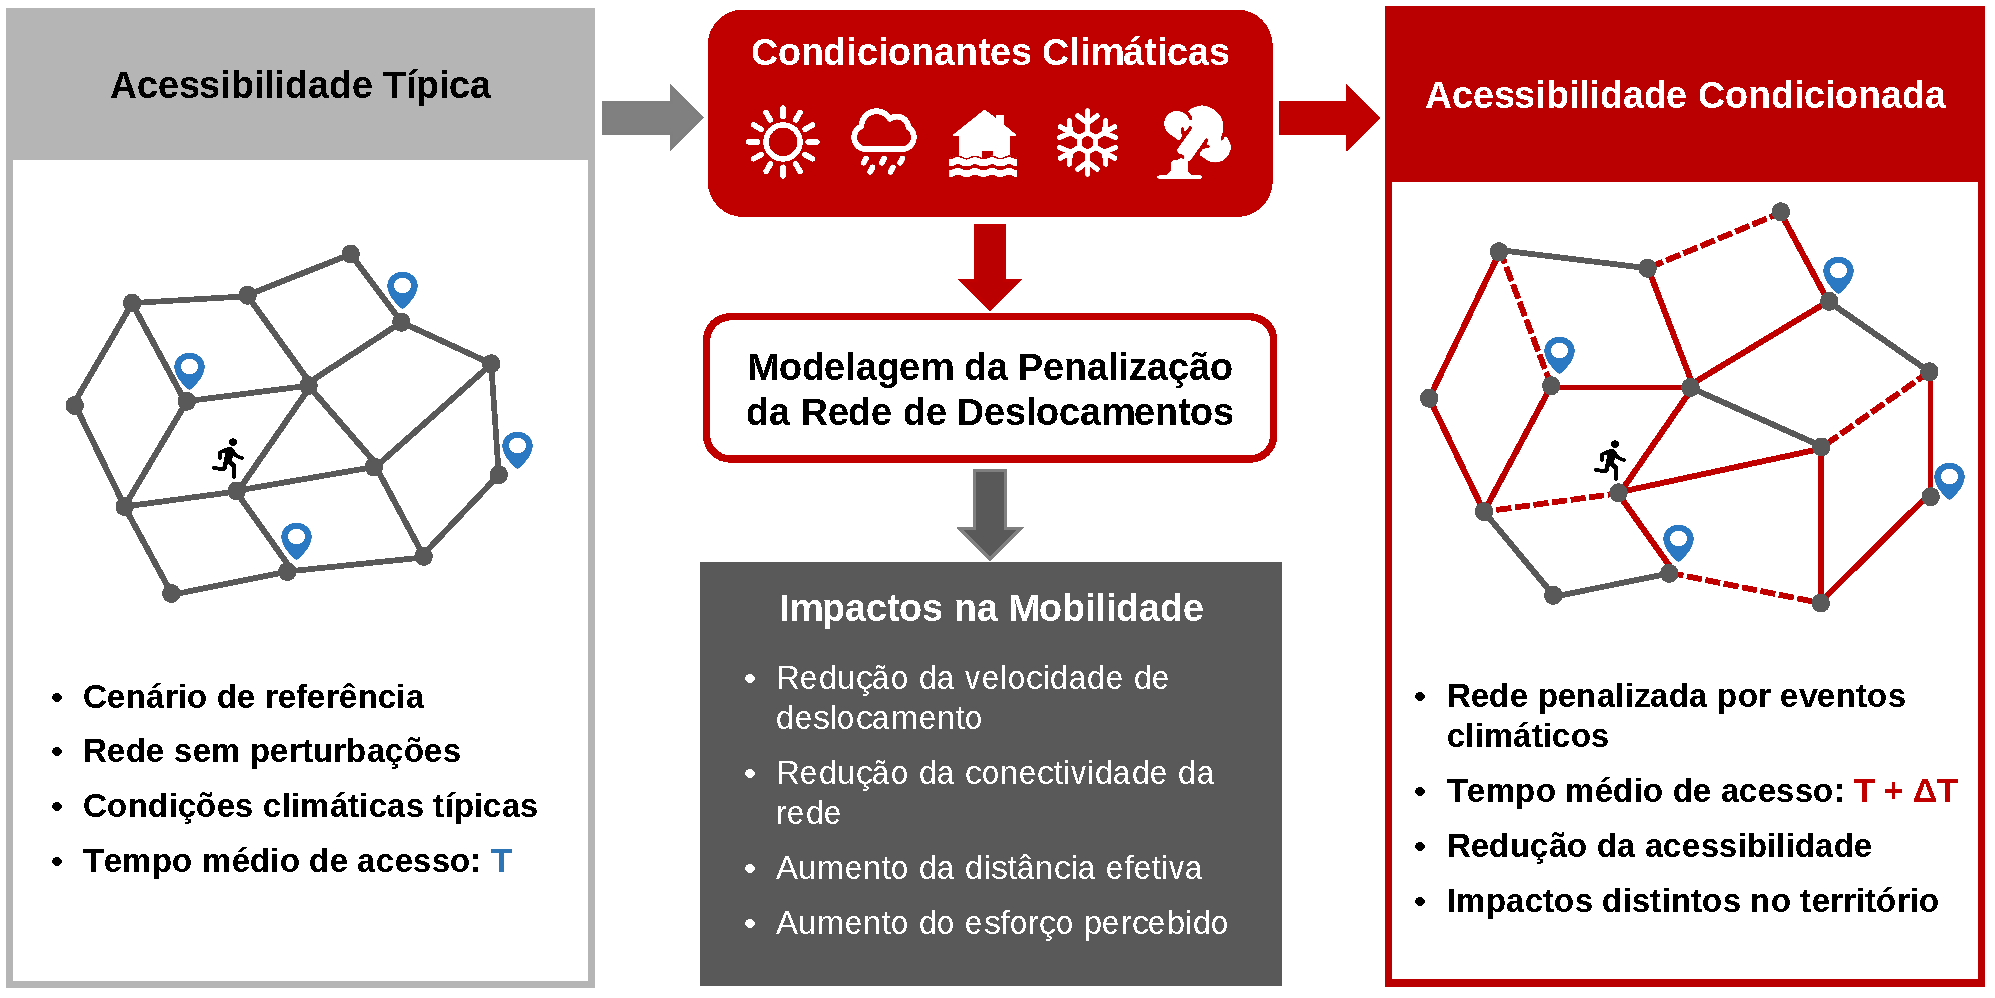
\includegraphics[width=1\textwidth]{figs/framework.pdf}
  \caption{Modeling flow for accessibility scenarios. Edges lengthen as their travel cost increases, so the geometry in the right panel encodes the effect of the disruption rather than the physical street layout.}
  \label{fig:framework}
\end{figure}

\subsubsection{Territorial Modeling}
\label{subsec:territorial_modelling}

The urban territory is assembled from four data types that differ in geometry, resolution, and coordinate reference system, and whose integration is the first source of complexity in the pipeline.

\begin{description}
  \item[Analysis grid.] A regular partition of the territory defining the minimum unit of study. The library supports hexagonal and square cells; the side or radius is a parameter set according to the transport mode and the local context. With hexagonal cells, the distance between neighboring centroids is uniform in all six directions, which avoids the directional bias that square cells introduce in neighborhood-based aggregation. The centroid of each cell is the theoretical origin of trips and the basis for computing and aggregating indicators.
  \item[Points of interest (POIs).] The destinations of trips: coordinates locating the everyday services used by the population, organized into categories such as health, education, and transport. Their selection depends on the availability of local databases, whether official or crowdsourced. Each POI is snapped to the nearest network vertex before routing, so the reachable set is bounded by the network rather than by straight-line distance.
  \item[Street network.] The mobility infrastructure is structured as a spatial graph, with vertices at intersections and edges along street segments whose initial base weight is travel time. Each cell centroid is attached to the nearest network vertex, and a maximum snap distance discards cells whose centroid lies too far from the network — a parameter that prevents a cell in an unmapped area from being routed through a vertex several kilometers away. Because this threshold removes cells from the analysis, it must be reported alongside the results.
  \item[Environmental layers.] Spatial layers that may be continuous, such as raster images, or discrete, such as vector polygons, mapping the climate or environmental phenomena under evaluation. A single scenario may stack several such layers. They are overlaid on the street network to adjust the travel cost of affected edges, as described in Section~\ref{sec:penalization}.
\end{description}

A fifth input completes the model. \textbf{Demographic and socioeconomic data} characterize the resident population — density, income, and schooling — and come from official censuses. These data are published in irregular administrative units such as census tracts, which do not align with the analysis grid, so each tract attribute is transferred to the cells by area-weighted mean: a cell receives the average of the tract values covering it, weighted by the intersected area. Where a tract has no value, its area is excluded from the denominator, so a cell partially covered by suppressed data is not diluted toward zero. The numerator and denominator are both taken from tracts with data, which keeps the cell value equal to the value of its contributing tracts rather than to a fraction of it.

This distinction between interpolation by density and aggregation by area is not interchangeable. Density interpolation conserves totals and suits population counts; area-weighted averaging preserves the value of the attribute itself and suits rates and indices. Population is interpolated the first way, socioeconomic indices the second.

\subsection{The Cost-Modification Mechanism}
\label{sec:penalization}

The framework fixes neither which environmental variables alter the network nor the magnitude of their effect. It exposes a \emph{mechanism} that receives environmental layers and returns a new cost for each edge; selecting the layers and setting their parameters belongs to whoever applies the method. This section describes that mechanism.

\subsubsection{Scenarios}

The network is evaluated in two states. In the \textbf{typical scenario}, each edge weight ($W_{base}$) is the travel cost under normal conditions — the segment length divided by the mean speed adopted for the mode under analysis. In the \textbf{conditioned scenario}, weights are recomputed from the environmental layers ($C$), producing $W_{cond}$ for each edge.

Comparing the two states isolates the effect of the disruption: any difference in accessibility indicators is attributed to the cost change introduced by the environmental layers.

\subsubsection{Cost modifiers}

The core element of the mechanism is the \emph{cost modifier}. Each modifier is a function that takes the value of a layer at a point on the edge and returns a multiplicative factor:

\begin{equation}
  f(v) \rightarrow \mathbb{R}^{+}
\end{equation}

where $v$ is the value sampled from the layer at that point. The factor $f$ may exceed 1 (penalization), fall below 1 (attenuation), or be infinite (interdiction). The same mechanism covers all three cases, which is why the framework refers to \emph{cost modifiers} rather than penalties alone.

A modifier never receives the whole edge: it is applied to values sampled along it. Sampling strategy and factor aggregation are declared separately, so phenomena with different spatial distributions are handled by the same mechanism.

\subsubsection{Sampling}

Two sampling strategies are available, and the choice trades cost for fidelity. \textbf{Midpoint} queries the layer at the edge midpoint and applies a single factor to the entire edge, which is fast but inaccurate when the edge crosses a boundary. \textbf{Segments} places $n$ equidistant points along the edge, including both endpoints, and reads the layer at each; the value of $n$ is a parameter, defaulting to four.

The distinction matters most for long edges, which are common in peripheries where blocks are large. A single edge can span several hundred meters and cross more than one thermal or topographic zone. Sampling only its midpoint may place the entire segment in the wrong class.

\subsubsection{Reading the layers}

How a layer is queried depends on the nature of the data.

\textbf{Continuous data} (rasters) are sampled at the chosen points. Each point takes the value of the pixel containing it. Points landing on a nodata pixel leave the cost unchanged at that location rather than propagating a missing value into the cost, so an incomplete raster degrades coverage instead of corrupting the network.

\textbf{Discrete data} (vector polygons) are queried by intersection. The edge is partitioned at every point where a polygon boundary crosses it, and each resulting sub-segment receives the factor of the polygon covering it. Sub-segments outside any polygon keep the original cost. Where polygons overlap, the \emph{largest} factor among them applies to the overlap, so a region mapped by two hazard layers is governed by the more restrictive one.

\subsubsection{Aggregation and interdiction}

The factors obtained along an edge must be reduced to a single value for the whole edge. The framework offers two reductions:

\begin{itemize}
  \item \textbf{Maximum}: adopts the most restrictive factor observed along the segment, treating the edge by its worst case. This is conservative and appropriate when the sample is small.
  \item \textbf{Length-weighted mean}: each sub-segment pays its own factor, and the mean is weighted by extent. This is more faithful on long edges crossing heterogeneous regions.
\end{itemize}

Infinite factors receive separate treatment. Assigning $f = \infty$ to a sub-segment declares it impassable: the cost of any path crossing it becomes infinite, and routing prefers alternatives. Interdiction is not a high cost but a statement that crossing is not viable in that scenario — the appropriate treatment for phenomena that block the road rather than delay it, such as a landslide burying the segment. When no alternative exists, the cell reaches no destination at all, a situation recorded as access loss.

\subsubsection{Composition}

When more than one environmental layer affects the same edge, modifiers are applied in sequence and the result accumulates multiplicatively:

\begin{equation}
  W_{cond} = W_{base} \times f_1 \times f_2 \times \cdots \times f_n
\end{equation}

Each step receives the cost produced by the previous one. Because multiplication commutes, the order does not change the numeric result, but it changes how the process reads, which matters when attributing an accessibility change to a specific layer.

This composition admits two arrangements. In \emph{simple rules}, each modifier queries one layer independently and chaining happens across rules. In \emph{composite rules}, several layers are queried at the same point on the edge and the factor is computed jointly, allowing one layer's effect to depend on another's value.

The distinction is not cosmetic. In the simple arrangement, an attenuation by vegetation would apply to any tree-lined segment, including where there is no heat at all — dense canopy next to a shaded, cool street would still receive a discount. In the composite arrangement, vegetation attenuates only where the thermal layer exceeds a threshold at that same point, so the two factors are evaluated jointly rather than independently averaged. A composite rule thus samples all its layers at identical locations before aggregating, preserving the spatial correspondence between their values.

\subsubsection{Recalculation and indicators}

With conditioned costs defined, a least-cost path algorithm runs over the graph, producing travel-time matrices for both scenarios. From these, the indicators described in Section~\ref{subsec:territorial_modelling} are computed: the mean time to reach the $k$ nearest POIs of each category (PTh), the inequality of its distribution (index G), and the share of the population served within a threshold (F15).

The scenario comparison adds per-cell time variation and \emph{access loss}: cells reaching no POI under the conditioned scenario receive infinite time and are accounted for separately. They are not an extreme case of high time but the absence of access, and treating them as a numeric value would distort any mean or inequality index computed over the remainder.

\subsection{Applicability}
\label{subsec:applicability}

This section states the criterion by which the scenarios were selected. The mechanism must handle environmental evidence in several forms, and each scenario instantiates one of them.

\subsubsection{Selection Criterion}

The mechanism varies along three axes: whether the environmental layer is continuous or discrete, whether several layers are read independently or jointly at the same location, and whether the effect is a penalization or an interdiction. Each scenario instantiates one combination of these values, and the set was chosen so that each axis appears at both of its values.

Several scenarios run on the same city and differ only in the layers they declare, so the variation in behavior follows from configuration.

\subsubsection{Coverage of the Mechanism}

Table~\ref{tab:cenarios} lists the seven conditioned scenarios by the capability each exercises.

\begin{table}[H]
\centering
\footnotesize
\caption{Scenarios by the capability of the mechanism they exercise}
\label{tab:cenarios}
\begin{tabularx}{\linewidth}{|l|l|X|l|}
\hline
\textbf{Scenario} & \textbf{Layers} & \textbf{Capability exercised} & \textbf{Effect} \\
\hline
\texttt{thermal} & 1 raster & Sampling of a continuous field & penalization \\
\texttt{thermal+green} & 2 rasters, joint & Composite rule over co-located layers & penalization \\
\texttt{thermal\_demo} & 1 raster & Response to a steeper gradient & penalization \\
\texttt{thermal+green\_demo} & 2 rasters, joint & Composite rule under a steeper gradient & penalization \\
\texttt{flood} & 1 vector & Partition at polygon boundaries & penalization \\
\texttt{landslide} & 1 vector & Same, with infinite factors & interdiction \\
\texttt{flood+landslide} & 2 vectors & Sequential composition, interdiction dominates & both \\
\hline
\end{tabularx}
\end{table}

Three properties follow from the table.

\textbf{Both branches of the modifier are exercised.} Curitiba samples continuous fields and Porto Alegre intersects polygon geometries, which are distinct implementation paths.

\textbf{Both outcomes of the cost function are exercised.} Flooding raises travel cost while preserving every connection, so all paths exist in both scenarios with a different weight. Landsliding makes segments impassable, and some origins lose access entirely. The framework reports the second separately, since it is an absence of access and not a slowdown.

\textbf{Composition appears in homogeneous and sequential form.} The \texttt{thermal+green} scenario reads two rasters at identical sampled points and returns a single factor, the thermal one multiplied by the shading reduction wherever vegetation is present. Sampling both layers at the same position is what requires a composite rule: two chained simple rules would each sample the segment independently and could read vegetation at a point whose temperature was read elsewhere. The \texttt{flood+landslide} scenario applies two vector rules in sequence, and the interdiction of one dominates the penalization of the other on shared edges.

\subsubsection{Demonstrative Scenarios}

Two Curitiba scenarios use a thermal coefficient roughly seven times the calibrated value. They are demonstrative, and the text does not read them as estimates. Their purpose is to show that the mechanism responds monotonically to the magnitude of its input: a steeper gradient that produced a smaller accessibility change would indicate a defect in the composition. Reporting them alongside the calibrated scenarios makes the sensitivity of the pipeline observable at no additional cost, since they differ only in a parameter.
\subsubsection{Scope and Limitations}

Two limits follow from the design and belong alongside the results.

\textbf{The mixed representation is supported at the component level.} The implementation reads a raster and a vector at the same sample point, and tests cover this path, but no scenario here declares one of each. Doing so requires a study area where both evidence types describe the same phenomenon, which the two municipalities do not provide.

\textbf{The estimates await validation against observations.} Accessibility under a hypothetical disruption has no measured counterpart, since the conditioned scenario did not occur. This work establishes that the mechanism computes what it specifies and that the framework accommodates disruptions of different forms. Matching the resulting travel times to what pedestrians would experience requires observed mobility under an actual event.

Together these limits place the contribution: a framework demonstrated to be applicable across representations and outcomes. Empirical validation of its predictions remains open.

